\section{Case study}
\label{caseStudy}
\subsection{Scenario Description}
Passing manuever is scenario on 2 lane road, target vehicle, 1 environmental vehicle. The target vehicle must perform a lane change maneuver in order to get into the left turn lane before the end of the scenario.
\begin{figure}[tb]
	\label{fig:discreteview}
		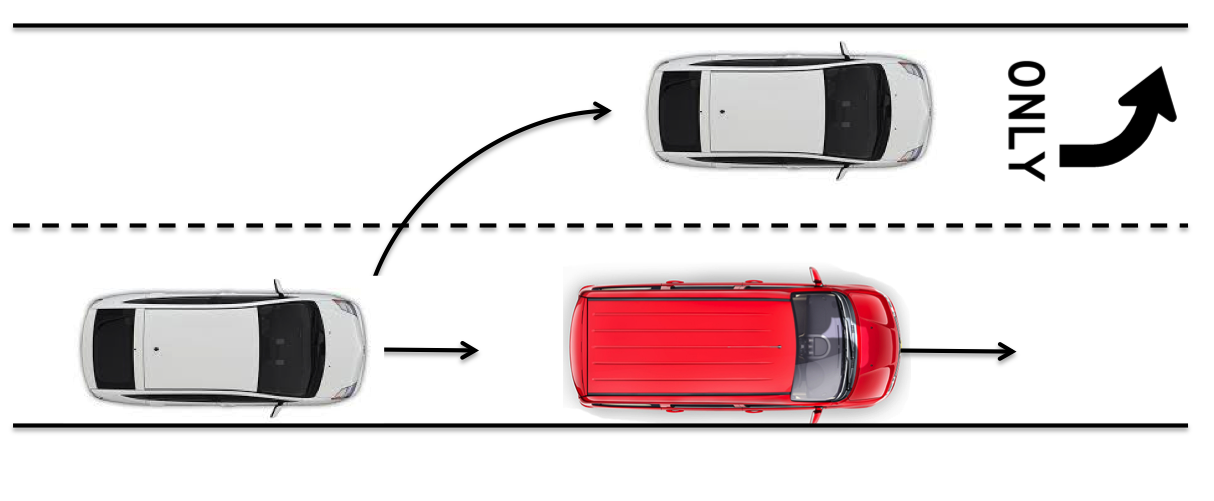
\includegraphics[scale=.4]{scenario.png}
	\caption{Pictorial description of target vehicle scenario}
\end{figure}
\subsection{Target Vehicle Model}
\begin{enumerate}
	\item Target vehicle has non linear dynamics described by bicycle model.
	\item Trajectories are defined for right to left lane switch and left to right lane switch.
	\item Hybrid system modes are described by drive forward and lane change.
	\begin{enumerate}
		\item Lane change is hierarchical and has sub-modes, right to left, straight, and left to right.
		\item Each submode has same dynamics but implements a different motion primitive.
	\end{enumerate}
	\item Target vehicle has non linear dynamics described by bicycle model.
	Consider the target vehicle defined as a non-linear hybrid system using a  bicycle model:
	\begin{equation}
	\begin{aligned}
	\ddot{\beta}=\left(\frac{C_rl_r-C_fl_f}{mv^2} \right)\dot{\psi}+\\
	\left(\frac{C_f}{mv} \right)\delta-\left(\frac{C_f+C_r}{mv} \right)\beta+y_{\beta}
	\end{aligned}
	\end{equation}
	\begin{equation}
	\begin{aligned}
	\ddot{\psi}=\left(\frac{C_rl_r-C_fl_f}{I_z} \right)\beta-\\
	\left(\frac{C_fl_f^2-C_rl_r^2}{I_z} \right)\left(\frac{\dot{\psi}}{v} \right)+
	\left(\frac{C_fl_f}{I_z} \right)\delta+y_{\dot{\psi}}
	\end{aligned}
	\end{equation}
	\begin{equation}
	\dot{v}=a_x+y_v
	\end{equation}
	\begin{equation}
	\dot{s_x}=v\cos{\beta+\psi}+y_{s_x}
	\end{equation}
	\begin{equation}
	\dot{s_y}=v\sin{\beta+\psi}+y_{s_y}
	\end{equation}
	\begin{equation}
	\dot{\delta}=v_w+y_d
	\end{equation}
	
	\(C_f,C_r\) and \(l_f, l_r\) describe respectively the cornering stiffness and distances from the center of gravity to the axles. \(I_z\) is the moment of inertia and \(m\) is the vehicle mass. \(\beta\) is the slip angle at the center of mass, \(\psi\) is the heading angle, \(\dot{\psi}\) is the yaw rate, \(v\) is the velocity, \(s_x\) and \(s_y\) are the x and y positions, and \(\delta\) is the angle of the front wheel. In the formulation of [6], the inputs to the system are \(a_x\), the logitudinal acceleration, and \(v_w\) the rotational speed of the steering angle. The \(y\) terms represent disturbances to the system. For example \(y_{\beta}\) and \(y_{\dot{\psi}}\) represent disturbances to the slip angle at the center of mass and the yaw rate. 
	\item Trajectories are defined for right to left lane switch and left to right lane switch.
	\item Hybrid system modes are described by drive forward and lane change.
	\begin{enumerate}
		\item Lane change is hierarchical and has sub-modes, right to left, straight, and left to right.
		\item Each submode has same dynamics but implements a different motion primitive.
	\end{enumerate}
\end{enumerate}
\subsection{Environmental Vehicle Model}
Environmental vehicle has simple 2D dynamics, no specific controller, non-determinism describes state evolution.
\begin{enumerate}
	\item Environmental vehicle must drive forwards.
	\item Environmental vehicle must not change lanes if other lane is occupied.
	\item At every step the environmental vehicle can apply +/- some specified level of acceleration.
	\item At every step environmental vehicle can switch lanes if condition 2 is not violated.
\end{enumerate}
Environmental vehicle has simple 2D dynamics, no specific controller, non-determinism describes state evolution.
\begin{enumerate}
	\item Environmental vehicle must drive forwards.
	\item Environmental vehicle must not change lanes if other lane is occupied.
	\item At every step the environmental vehicle can apply +/- some specified level of acceleration.
	\item At every step environmental vehicle can switch lanes if condition 2 is not violated.
\end{enumerate}
\subsection{dReal Model}
\begin{enumerate}
	\item 1 or 2 modes depending on lane change or passing.
	@@ -28,5 +27,4 @@ Passing manuever is scenario on 2 lane road, target vehicle, 1 environmental veh
	\item Plant controller is tracking controller which follows trajectory.
\end{enumerate}
\subsection{Controller with Partial Dynamics}
A finite transition system describing the passing manuever is given in UPPAAL (or NuSMV).
\begin{figure}[tb]
	\label{fig:discreteview}
	\centering
	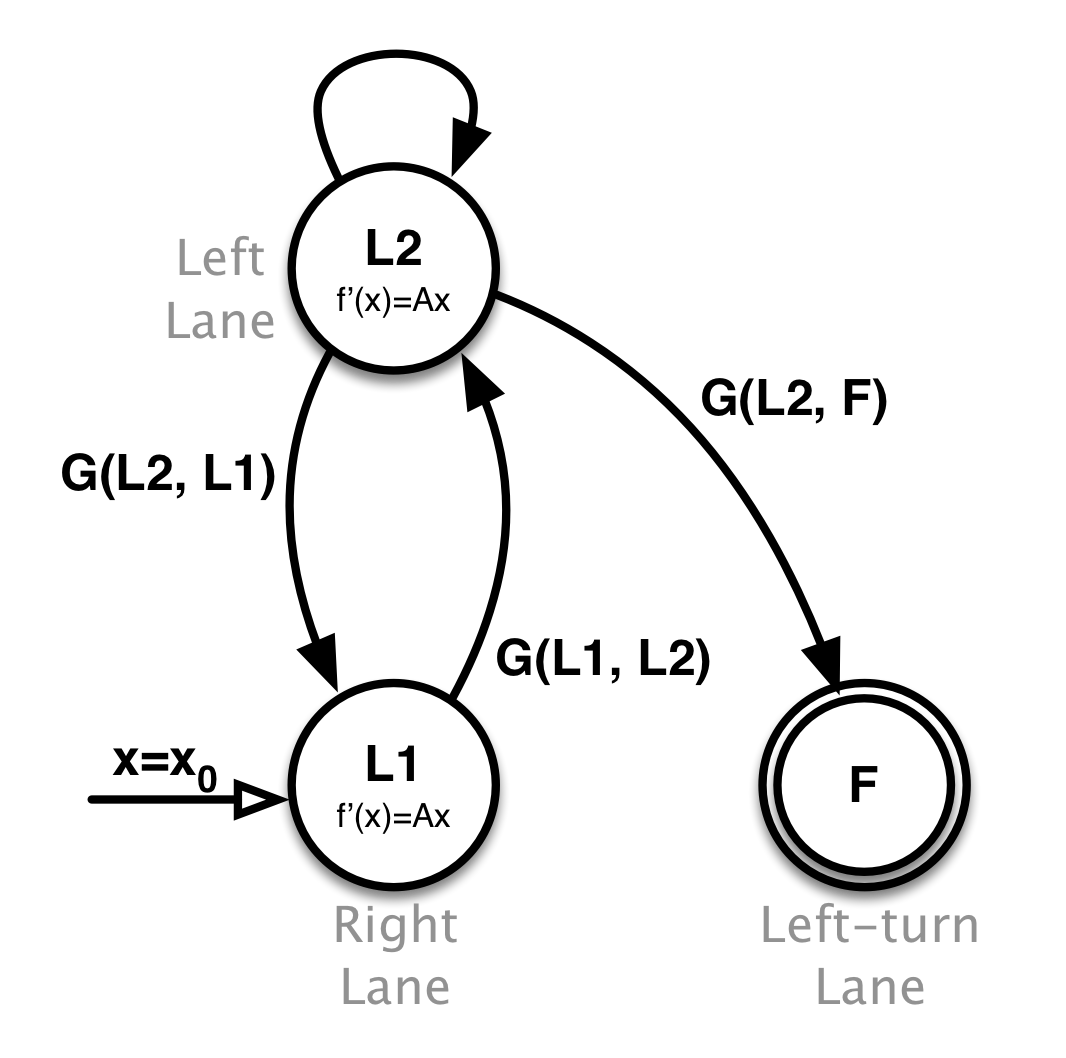
\includegraphics[scale=.7]{lane_change_timed.png}
	\caption{Automata with partial dynamics describing scenario}
\end{figure}